\documentclass{beamer}
%\usepackage[urlcolor=blue]{hyperref}
\definecolor{links}{HTML}{2A1B81}
\hypersetup{colorlinks,linkcolor=,urlcolor=blue}
\usepackage[utf8]{inputenc}
\usepackage[spanish]{babel}
\usepackage{graphicx}
\usepackage{ragged2e}
\usepackage{xcolor}
            
\newcommand{\toRight}[1]{
    \begin{FlushRight}
        {\tiny #1}
    \end{FlushRight}
} % Align to right

\title{Database Administration: The Complete Guide to Practices and Procedures}
\subtitle{Chapter 1: Introduction - What is a DBA?}
\author{Andrés Calderón}
\date{\today}

\begin{document}

\frame{\titlepage}

\section{Conceptos Básicos}

\begin{frame}{Qué es una base de datos?}
    \begin{itemize}
        \item Una base de datos es un almacén organizado de datos en el que los datos son accesibles por elementos de datos con nombre. 
        \item Un DBMS es un software que permite a los usuarios finales o programadores de aplicaciones compartir datos.
        \item Proporciona un método sistemático para crear, actualizar, recuperar y almacenar información en una base de datos.
    \end{itemize}
    \toRight{Appendix 1, “Database Concepts and Fundamentals.”}
\end{frame}

\begin{frame}{Qué es una base de datos?}
    \begin{itemize}
        \item Los DBMS también son generalmente responsables de la integridad de los datos, la seguridad de los datos, el control y la optimización del acceso a los datos, la reversión automatizada, el reinicio y la recuperación. 
        \item En términos simples, puede pensar en una base de datos como una carpeta de archivos. Puede pensar en el archivador que contiene los archivos junto con las etiquetas de archivo como DBMS.
    \end{itemize}
    \toRight{Appendix 1, “Database Concepts and Fundamentals.”}
\end{frame}

\begin{frame}{Funciones del DBMS}
    \begin{itemize}
        \item Mantener la integridad de los datos.
        \item Garantizar la seguridad de los datos.
        \item Optimizar el acceso a los datos.
        \item Proveer reversión automatizada, reinicio y recuperación.
    \end{itemize}
\end{frame}

\begin{frame}{\_}
    \begin{tabular}{c}
        DBMS vs Database \\
        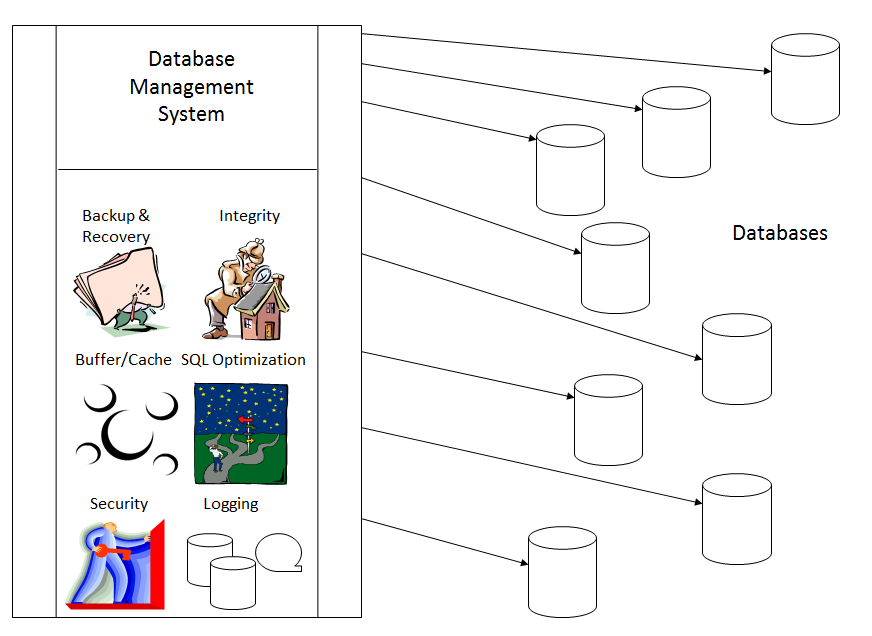
\includegraphics[width=0.9\textwidth]{figures/dbms_vs_database.png}
    \end{tabular}
    \toRight{\url{http://thedatabasesite.com/page100.html}}
\end{frame}

\section{Porqué aprender Administración de Bases de Datos?}

\begin{frame}{Porqué ser un DBA?}
    \begin{itemize}
        \item Diseñar y mantener las bases de datos de una empresa.
        \item Estar en el centro de los negocios.
        \item Aprender sobre nuevas tecnologías.
        \begin{itemize}
            \item Además de tener la oportunidad de aprender sobre muchas facetas de los negocios y cómo las empresas utilizan los datos.
        \end{itemize}
    \end{itemize}
\end{frame}

\begin{frame}{Qué hace a un buen DBA?}
    \begin{itemize}
        \item Solucionador de problemas.
        \item Disfruta de los desafíos.
        \item Aprendizaje constante.
        \item Puede trabajar solo o en equipo.
        \item Experiencia como programador.
    \end{itemize}
\end{frame}

\begin{frame}{Generalmente los DBAs obtienen buena remuneración por su trabajo...}
    \begin{itemize}
        \item According to a salary study conducted by Global Knowledge and TechRepublic the average DBA salary is \$78,468, while their managers average \$87,261. 
        \begin{itemize}
            \item For full-time employees functioning as a DBA, the mean salary ranges in the high \$80 thousands
        \end{itemize}

        \item According to the Dice 2010-11 Tech Salary Survey, Oracle experience is requested in more than 15,000 job postings on any given day. 
        \begin{itemize}
            \item Demand for Oracle skills is up 57\% year over year, and the national average salary for technology professionals with experience in Oracle Database is \$90,914. 
        \end{itemize}

        \item The BLS (May 2010) reports that the median annual wage of database administrators was \$73,490 and the mean annual wage was \$75,730. 
    \end{itemize}
\end{frame}

\begin{frame}{Generalmente los DBAs obtienen buena remuneración por su trabajo...}
    \noindent 
    \begin{minipage}{0.45\textwidth}
        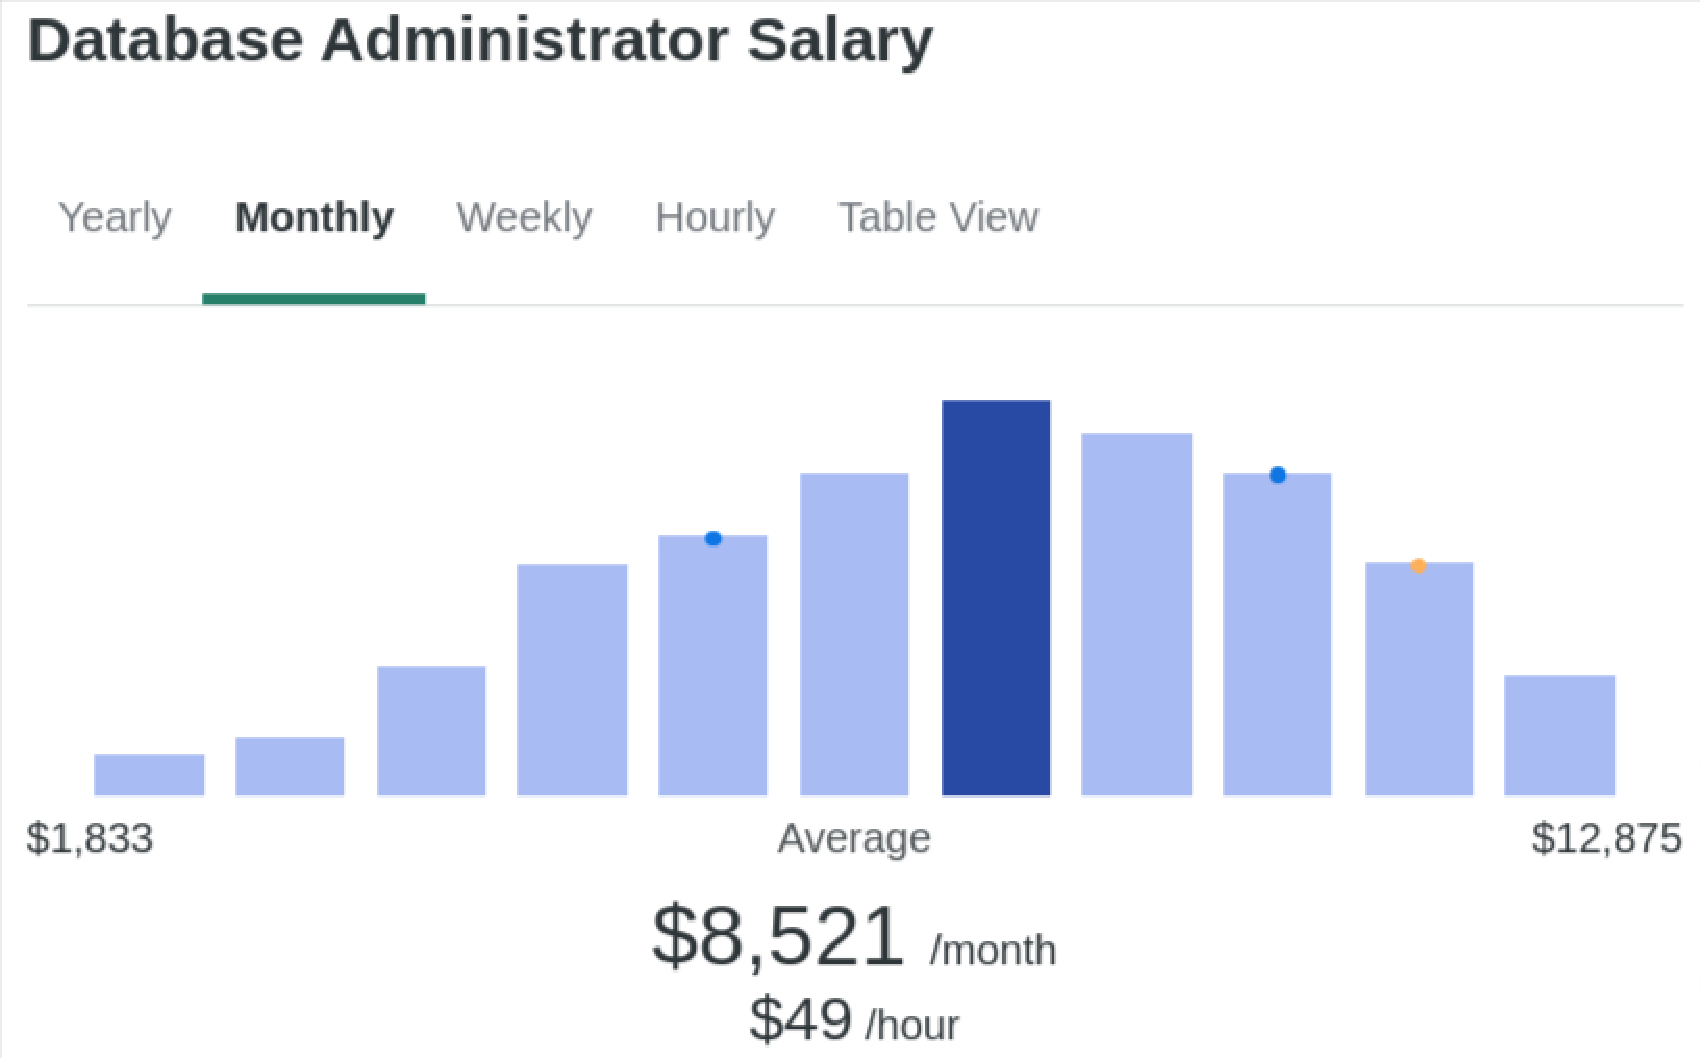
\includegraphics[width=\textwidth]{figures/dba_salary_plot}
    \end{minipage}
    \hspace{0.05\textwidth}
    \begin{minipage}{0.45\textwidth}
        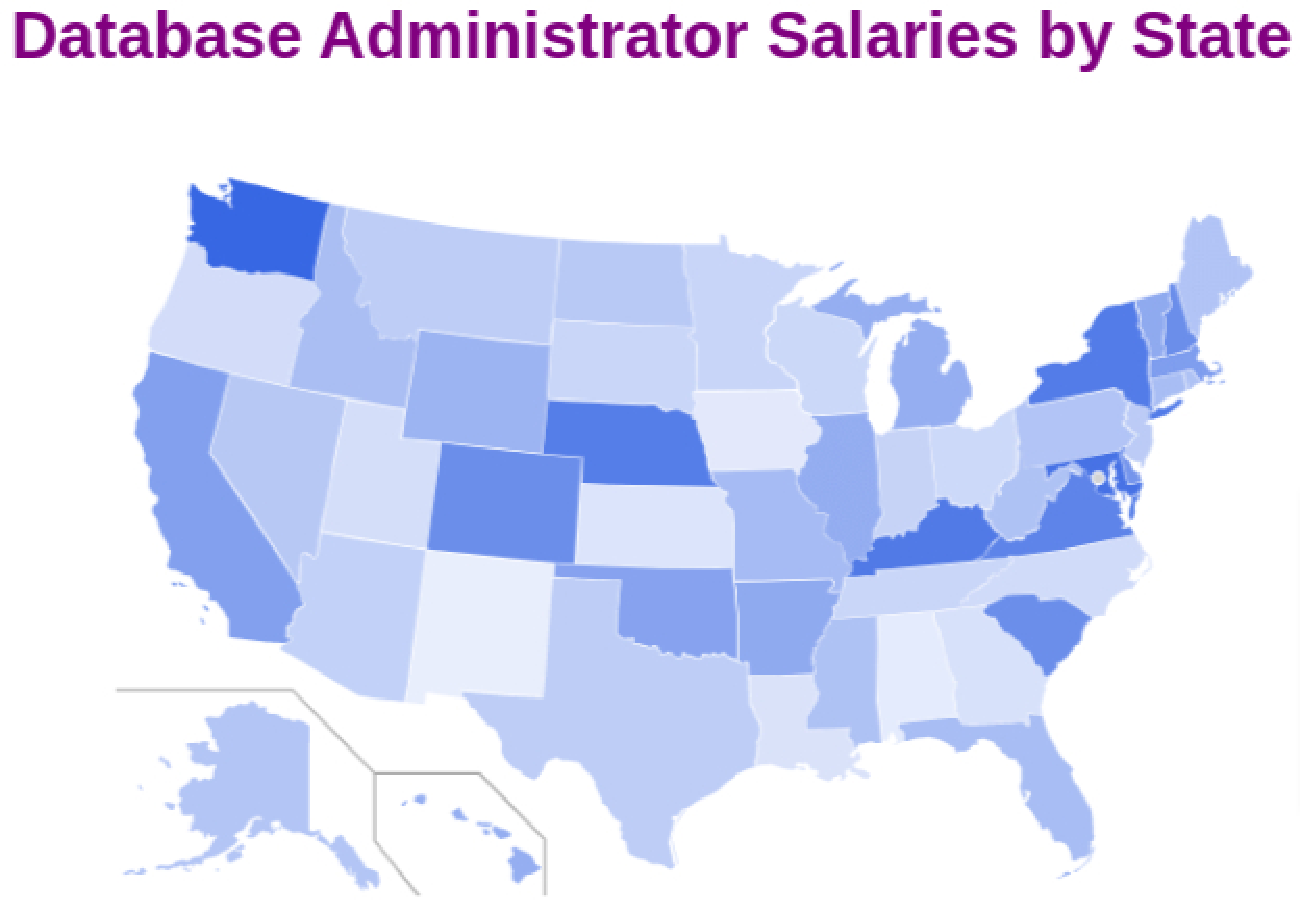
\includegraphics[width=0.9\textwidth]{figures/dba_salary_map}
    \end{minipage}%
    \vspace{5mm}
    Recursos adicionales:
    \begin{enumerate}
        \item \href{https://www.cs.ucr.edu/~acald013/public/Javeriana/DBA_Salary.html}{Estadísticas actuales} en US, Europa, Latinoamérica y Colombia.
        \item Diferentes \href{https://www.cs.ucr.edu/~acald013/public/Javeriana/Certifications.html}{tipos de certificaciones.}
    \end{enumerate}

\end{frame}

\begin{frame}{Desventajas de ser un DBA...}
    \begin{itemize}
        \item Los DBA están bien pagados, son altamente empleables, poseen trabajos desafiantes y es probable que participen en los proyectos más visibles e importantes. Pero...
        \item Se espera que los administradores de bases de datos sepan todo, no solo sobre la tecnología de bases de datos, sino sobre cualquier cosa conectada a ella. 
        \item Los DBA casi nunca trabajan días de 8 horas, sino que trabajan largas jornadas con muchas horas extras, especialmente cuando el rendimiento está sufriendo o los proyectos de desarrollo están retrasados. 
    \end{itemize}
\end{frame}


\begin{frame}{Desventajas de ser un DBA...}
    \begin{itemize}
        \item Según los analistas de la industria, el DBA promedio trabaja más de 50 horas por semana.
        \item Los administradores de bases de datos con frecuencia tienen que trabajar los fines de semana y días festivos para mantener las bases de datos durante las horas de menor actividad.
    \end{itemize}
\end{frame}

\begin{frame}{The Management Discipline of Database Administration}
    \begin{itemize}
        \item Un DBA es el técnico de información responsable de garantizar la funcionalidad operativa continua y la eficiencia de las bases de datos de una organización y las aplicaciones que acceden a esas bases de datos.
    \end{itemize}
    
    \toRight{\url{http://datatechnologytoday.wordpress.com/2011/02/27/dba-as-a-management-discipline/}}
\end{frame}

\section{Roles y Responsabilidades}

\begin{frame}{Roles y Responsabilidades}
    \begin{tabular}{c}
        Database, Data, and System Administration \\
        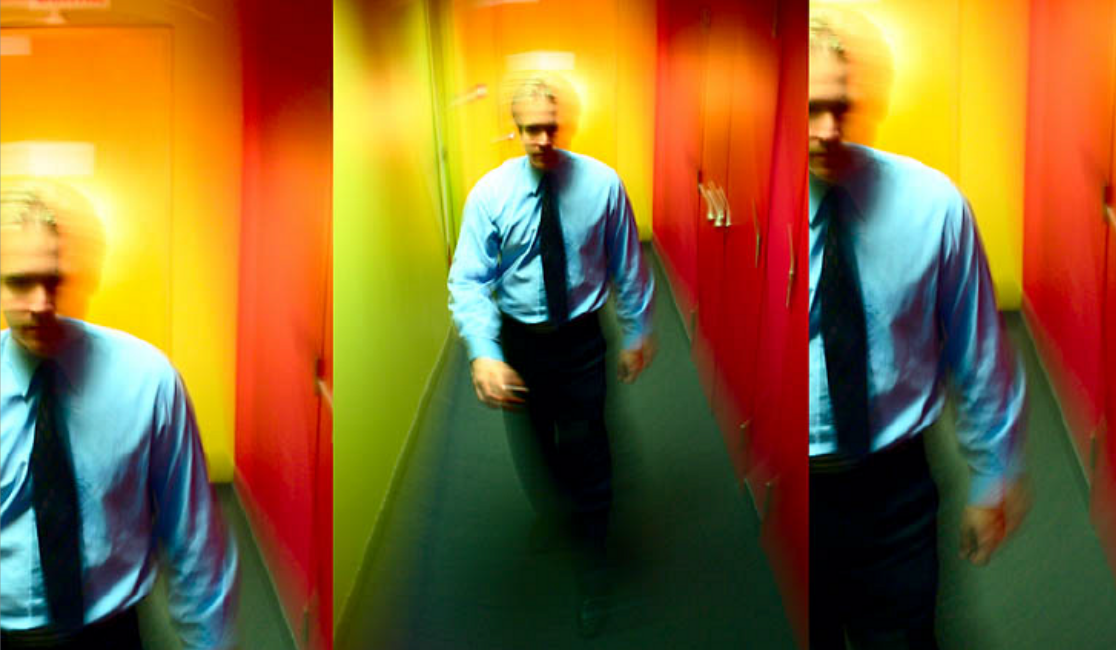
\includegraphics[width=0.9\textwidth]{figures/DDS.png}
    \end{tabular}
\end{frame}

\begin{frame}{Database, Data, and System Administration}
    \begin{itemize}
        \item Algunas organizaciones definen roles separados para los aspectos empresariales de los datos y los aspectos técnicos de los datos.
        \item Los aspectos de negocio de los datos están alineados con una disciplina conocida como administración de datos, mientras que los aspectos más técnicos son manejados por la administración de bases de datos. 
    \end{itemize}
\end{frame}

\begin{frame}{Database, Data, and System Administration}
    \begin{itemize}
        \item No todas las organizaciones tienen una función de administración de datos. De hecho, muchas organizaciones combinan la administración de datos en el rol de administración de bases de datos. 
        \item A veces, las organizaciones también dividen los aspectos técnicos de la gestión de datos, con el DBA siendo responsable de usar el DBMS y otro rol, conocido como administración del sistema o programación de sistemas, siendo responsable de instalar y actualizar el DBMS.
    \end{itemize}
\end{frame}

\begin{frame}{Data Administrator (DA) or Chief Data Officer (CDO)}
    \begin{itemize}
        \item No sobre tecnología, sobre datos y su significado en la organización...
        \item Responsable de reunir a la organización para tratar los datos como el activo corporativo que realmente es.
        \item Trata con metadatos y datos.
        \item Las organizaciones realmente preocupadas por la calidad, integridad y reutilización de los datos invariablemente implementarán y dotarán de personal la función de DA.
    \end{itemize}
\end{frame}

\begin{frame}{Metadata vs Data}
    \centering
    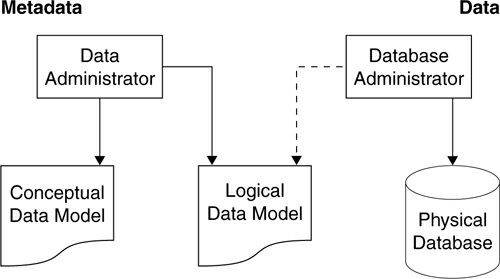
\includegraphics[width=0.75\textwidth]{figures/metadata2.png}
\end{frame}

\begin{frame}{System Administrator (SA)}
    \begin{itemize}
        \item Instalación y configuración de recursos informáticos.
        \item Tecnólogo puro.
        \item Sin responsabilidad por el diseño y soporte de la base de datos.
        \item Soporte de infraestructura.
        \item A veces llamado programador de sistemas.
    \end{itemize}
\end{frame}

\begin{frame}{Database Administrator (DBA)}
    \begin{itemize}
        \item Identifica y cataloga los datos requeridos por los usuarios empresariales.
        \item Produce modelos de datos conceptuales y lógicos para representar con precisión las relaciones entre los elementos de datos que ocurren dentro los procesos de negocio.
    \end{itemize}
\end{frame}

\begin{frame}{Database Administrator (DBA)}
    \begin{itemize}
        \item Produce un modelo de datos empresariales que incorpora todos los datos utilizados por todos los procesos de negocio de la organización.
        \item Configura las directivas de datos para la organización.
        \item Identifica propietarios, generadores y consumidores de datos.
        \item Establece estándares para el control y uso de datos.
    \end{itemize}
\end{frame}

\begin{frame}{Responsibilities}
    \centering
    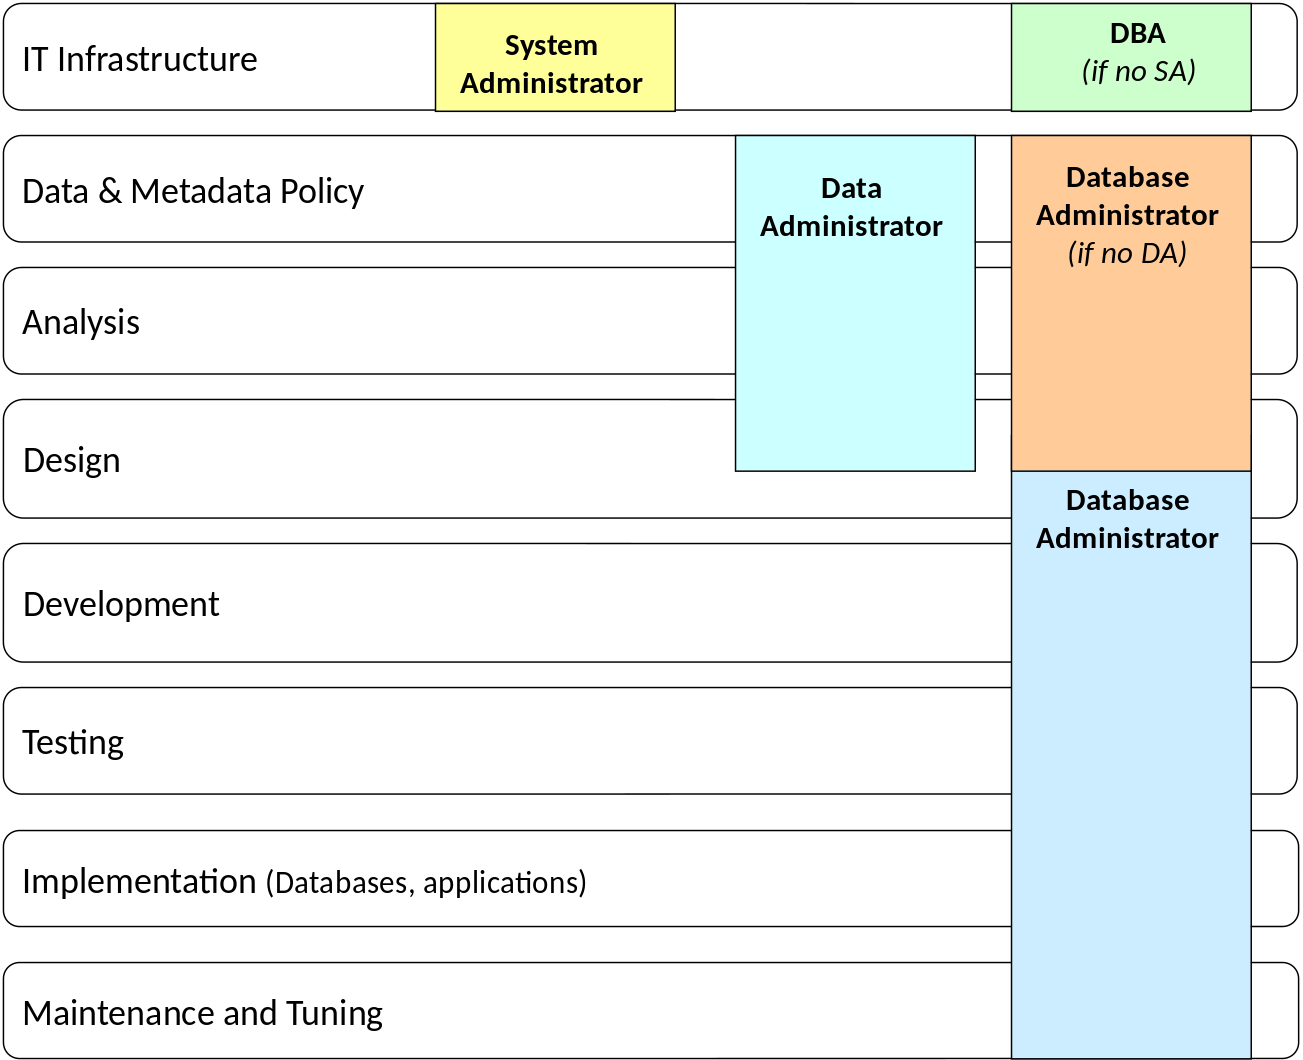
\includegraphics[width=0.9\textwidth]{figures/responsibilities.png}
\end{frame}

\begin{frame}{DBA Tasks}
    \centering
    Estas son las tareas de DBA necesarias para garantizar un entorno de base de datos óptimo para aplicaciones y usuarios:
    \begin{itemize}
        \item Crear el Ambiente o Entorno de las bases de datos.
        \item Diseñar las bases de datos.
        \item Diseñar aplicaciones que se conecten a las bases de datos.
        \item Revisar los diseños de las bases de datos.
        \item Liderar la gestión de cambios.
        \item Estar al tanto de la disponibilidad de los datos.
        \item Gestionar el desempeño.
        \begin{itemize}
            \item desempeño del sistema.
            \item desempeño de las bases de datos.
            \item desempeño de las aplicaciones asociadas.
        \end{itemize}
        \item Velar por la integridad de las bases de datos.
    \end{itemize}
\end{frame}

\begin{frame}{DBA Tasks}
    \centering
    Estas son las tareas de DBA necesarias para garantizar un entorno de base de datos óptimo para aplicaciones y usuarios:
    \begin{itemize}
        \item Estar al tanto de la seguridad de las bases de datos.
        \item Tolerancia a fallos, recuperación y copias de seguridad.
        \item Liderar planes de emergencia ante desastres.
        \item Gestión de almacenamiento.
        \item Mantenimiento y gestión de rutinas procedurales.
        \item Gestión de bases de datos distribuidas.
        \item Administración de Bodegas de Datos.
        \item Gerencia en las diferentes utilidades relacionadas a los SGBD instaladas.
        \item Conectividad a las diversas bases de datos.
        \item Cumplimiento normativo.
        \item Soft Skills!!!
    \end{itemize}
\end{frame}

\section{Conclusion}

\begin{frame}{Key Takeaways}
    \begin{itemize}
        \item Los DBA son esenciales para el funcionamiento de los datos empresariales.
        \item Trabajan con DA y SA para implementar y mantener bases de datos.
        \item Desempeñan un rol crítico en la eficiencia y seguridad de las bases de datos.
    \end{itemize}
\end{frame}

\end{document}
